\documentclass[a4paper,12pt, twoside]{book}
\usepackage{lmodern}
\newlength\longest
\usepackage{scrextend}
\usepackage{graphicx}
\usepackage[utf8]{inputenc}
\usepackage[T1]{fontenc} 
\usepackage{fouriernc}
\usepackage[document]{ragged2e}
\usepackage{amsmath}
\usepackage{amssymb}
\graphicspath{ {images/} }
\usepackage{hyperref}
\usepackage{macros}
\usepackage[normalem]{ulem}
\usepackage[]{algorithm2e}
\usepackage{pgf,tikz}
\usepackage{pgfplots}
\usepackage[signature=default_signature, date=01.06.2019]{mysignature}
\usetikzlibrary{spy}
\usetikzlibrary{backgrounds}
\usetikzlibrary{decorations.pathreplacing}
\usetikzlibrary{intersections}
\usepackage[margin=0.8in, right= 0.6in]{geometry}
\usepackage{textcomp}
\usetikzlibrary {automata,positioning}
%\usepackage {xcolor}
\definecolor {processblue}{cmyk}{0.96,0,0,0}
\usepackage{fancyhdr}
\pagestyle{fancy}
\fancyhead{}
\fancyhead[RO,LE]{Reachability Games with strong and relaxed energy constraints}
\fancyfoot{}
\fancyfoot[LE,RO]{\thepage}
\fancyfoot[LO,CE]{Chapter \thechapter}
\fancyfoot[CO,RE]{Ritam Raha}
\usepackage[nottoc,numbib]{tocbibind}
\usepackage{amsthm}
\theoremstyle{definition}
\newtheorem{theorem}{Theorem}[section]
\newtheorem{claim}[theorem]{Claim}
\newtheorem{conjecture}[theorem]{Conjecture}
\newtheorem{corollary}[theorem]{Corollary}
\newtheorem{definition}[theorem]{Definition}
\newtheorem{example}[theorem]{Example}
\newtheorem{fact}[theorem]{Fact}
\newtheorem{lemma}[theorem]{Lemma}
\newtheorem{proposition}[theorem]{Proposition}
\newtheorem{remark}[theorem]{Remark}

\begin{document}
\begin{titlepage}
	\centering
	\scshape 
	{\LARGE{CHENNAI MATHEMATICAL INSTITUTE}}\\
          \vskip 0.5cm
	MASTERS THESIS
	\vspace*{\baselineskip} 
	%------------------------------------------------
	%	Title
	%------------------------------------------------
	
	\rule{\textwidth}{1.6pt}\vspace*{-\baselineskip}\vspace*{2pt}
	\rule{\textwidth}{0.4pt} 

	\vspace{0.75\baselineskip}
	
	{\LARGE REACHABILITY GAMES WITH\\ strong and relaxed \\ ENERGY CONSTRAINTS\\} 
	
	\vspace{0.75\baselineskip} 
	
	\rule{\textwidth}{0.4pt}\vspace*{-\baselineskip}\vspace{3.2pt} 
	\rule{\textwidth}{1.6pt}
	
	\vspace{2\baselineskip} 
	
	%------------------------------------------------
	%	Author
	%------------------------------------------------
	
	
	
	\textit{Author:}
	
	\vspace{0.5\baselineskip} 
	
	{\scshape\Large Ritam Raha}\\ % Author
	\vspace{0.2\baselineskip}
	{\small Chennai Mathematical Institute}
	\vspace{2\baselineskip} 

		
	\textit{Supervised by:}     
	\vspace{0.5\baselineskip}

	{\scshape\Large Nicolas Markey}\ \ \ \ \&\ \ \ \  {\scshape\Large Loïc Hélouët}\\ % Supervisors
	\vspace{0.2\baselineskip}
	{\small INRIA Rennes}
	\vspace{2\baselineskip}

	\vspace{2\baselineskip} 
	
	\textit{A thesis submitted in fulfillment of the requirements\\ for the degree of Master of Science}\\
	\vspace{1\baselineskip}
	\textit{in the}\\
	\vspace{1\baselineskip}
	{\scshape Department of Computer Science\\ Chennai Mathematical Institute}

	\vspace{4\baselineskip}
	
	\includegraphics[width=0.7\textwidth]{cmi.png}

	\vfill % Whitespace between editor names and publisher logo
	
\end{titlepage}

\chapter*{Declaration}
I, Ritam RAHA, declare that this thesis titled, \textit{“Reachability Games with strong and relaxed energy constraints”} and the work presented in it are my own. I confirm that:
\vskip 1cm
\begin{itemize}
    \item This work was done wholly or mainly while in candidature for a masters degree(from CMI) at INRIA Rennes and CMI.
    \item The thesis has been prepared without resorting to plagiarism.
    \item Where I have consulted the published work of others, this is always clearly attributed.
    \item I have acknowledged all main sources of help.
    \item The thesis has not been submitted elsewhere for a degree.
\end{itemize}
\vskip 2cm
\mysignature[left]{full}

\chapter*{
%Quotes
}

\thispagestyle{empty}
\null\vfill

\settowidth\longest{\huge\itshape just as his inclination leads him;}
\begin{center}
\parbox{\longest}{%
  \raggedright{\huge\itshape%
   "The problem is \\ 
  not the problem; \\
  The problem is your attitude \\ 
  about the problem."\par\bigskip
  }   
  \raggedleft\Large\MakeUppercase{- Jack Sparrow}, \textit{Pirates of the Caribbean}\par%
}
\end{center}

\vfill\vfill

\chapter*{Abstract}
Quantitative reachability games are finite two player turn-based games played on weighted graphs. The objective of the game combines reachability objective(qualitative) with the (quantitative) requirement that the weights along a path must satisfy certain constraints (bounds). Besides having direct applications in reactive system synthesis with resource constraints, it is one of the simplest models that combine quantitative and qualitative objectives.
\vskip 0.5cm
In this thesis, we~first prove that under strict energy constraints (either only
lower-bound constraint or interval constraint), those games are
LOGSPACE-equivalent to energy games with the same energy constraints but without reachability objective (i.e., for infinite
runs). We~then consider two kinds of
relaxations of the upper-bound constraints (while keeping the
lower-bound constraint strict): in the first one, called \emph{weak
upper bound}, the upper bound is \emph{absorbing}, in the sense that
it allows receiving more energy when the upper bound is already
reached, but the extra energy will not be stored; in the second one,
we~allow for \emph{temporary violations} of the upper bound, imposing
limits on the number or on the amount of violations.

%
We prove that when considering weak upper bound, reachability
objectives require memory, but can still be solved in polynomial-time
for one-player arenas; we~prove that they are in coNP in the two-player
setting. Allowing for bounded violations makes the
problem PSPACE-complete for one-player arenas and EXPTIME-complete
for two players.

\chapter*{%Dedication}
}
I dedicate this to 
 


\chapter*{Acknowledgements}
I want to thank...

\tableofcontents

\chapter{Introduction}
\paragraph{Games on weighted graphs.}
Weighted games are a common way to formally address questions
related to consumption, production and storage of resources: the arena
of such game are two-player turn-based games in which transitions
carry positive or negative integers, representing the accumulation or
consumption of resource.  Various objectives have been considered for
such arenas, such as optimizing the total or average amount of
resources that have been collected along the play, or maintaining the
total amount within given bounds. The~latter kind of objectives,
usually referred to as \emph{energy
objectives}~\cite{CdAHS03,BouyerFLMS08}, has been widely studied in
the untimed
setting~\cite{ChatterjeeD12,ChatterjeeDHR10,DDGRT10,FahrenbergJLS11,JLR13,
JLS15,VCDHRR15,BMRLL15,BHMRZ17,DM18}, and to a lesser extent in the
timed setting~\cite{BFLM10,qest2012-BLM}.
%
As their name indicates, energy objectives can be used to model the
evolution of the available energy in an autonomous system: besides
achieving its tasks, the~system has to take care of recharging
batteries regularly enough so as to never run out of power.  Energy
objectives were also used to model moulding machines: such machines
inject molten plastic into a mould, using pressure obtained by storing
liquid in a tank~\cite{CJLRR09}; the~level of liquid has to be
controlled in such a way that enough pressure is always available, but
excessive pressure in the tank would reduce the service life of the valve.

Energy games impose strict constraints on the total amount of energy
at all stages of the play. Two kinds of constraints have been mainly
considered in the literature: lower-bound constraints (a.k.a. L-energy constraints) impose a strict lower bound (usually~zero), but impose no
upper bound; on~the other hand, lower- and upper-bound constraints
(a.k.a. LU-energy constraints) require that the energy level always
remain within a bounded interval~$[L;U]$. Finding strategies that
realize L-energy objectives along infinite runs is in PTIME in the
one-player setting, and in NP $\cap$ coNP for two players;
for LU-energy objectives, it~is respectively PSPACE-complete
and EXPTIME-complete~\cite{BouyerFLMS08}. Some works have also considered
the existence of an initial energy level for which a winning strategy
exist~\cite{ChatterjeeDHR10}.
%
Energy objectives have also been combined with other objectives,
either qualitative (e.g.~parity~\cite{ChatterjeeD12}) or quantitative
objectives (e.g.~multi-dimensional
energy~\cite{ChatterjeeDHR10,FahrenbergJLS11,JLR13}). 

In this paper, we focus on weighted games combining energy objectives
together with reachability objectives. Our~first result is the
(expected) proof that L-energy games with or without reachability
objectives are interreducible; the same holds for LU-energy games.

%
We~then focus on relaxations of the energy constraints, in two
different directions. In both cases, the lower bound remains
unchanged, as it corresponds to running out of energy, which we always
want to avoid. We~thus only relax the upper-bound constraint.
The~first direction concerns \emph{weak upper bounds}, already
introduced in~\cite{BouyerFLMS08}: in~that setting, hitting the upper bound
is allowed, but there is no overload, i.e. trying to exceed the upper bound will simply maintain the energy level at this maximal level. Yet, a strict lower bound is
still imposed. We~name these objectives LW-energy
objectives. This~could be used as a (simplified) model for batteries.
When considered alone, LW-energy objectives are not much different
from~ L-energy objectives, in the sense that the aim is to find a
reachable \emph{positive loop}. LW-energy games are in PTIME for
one-player games, and in NP $\cap$ coNP for two players. When
combining LW-energy and reachability objectives, the~situation
changes: different loops may have different effects on the energy
level, and we have to keep track of the final energy level reached
when iterating those loops.

The second way of relaxing upper bounds, which we call \emph{soft
upper bound}, allows a limited number (or amount) of
violations: when modeling a pressure tank, the lower-bound constraint
is strict (pressure should always be available) but the upper bound is
soft (excessive pressure may be temporarily allowed is
needed). We~consider different kinds of limits (on the number or
amount of violations), and prove that (with or without reachability
objectives) the energy game problems are PSPACE-complete for one-player arenas,
and EXPTIME-complete for two-player ones.

\fbox{minimization?}


\paragraph{Related work.}
Quantitative games have been the focus of numerous research articles
 since the~1970s, with various kinds of objectives. 
%such as ultimately
% optimizing the total payoff~\cite{}, mean-payoff~\cite{EM79,ZwickP95},
% or discounted sum~\cite{ZwickP95,Andersson06}.
% %
% Energy objectives, which are a kind of safety objectives on the total
% payoff, were introduced in~\cite{CdAHS03} and rediscovered
% in~\cite{BouyerFLMS08}.
% %
% Several works have extended those works by
% combining quantitative conditions together, e.g. multi-dimensional
% energy conditions~\cite{FahrenbergJLS11,JurdzinskiLS15} or
% conjunctions of energy- and mean-payoff
% objectives~\cite{ChatterjeeDHR10}. Combinations with qualitative
% objectives (e.g. reachability~\cite{Chatterjee0H17} or parity
% objectives~\cite{ChatterjeeD12,ChatterjeeRR14}) were also considered.
% %
% Similar objectives have been considered in slightly different
% settings e.g. Vector Addition Systems with States~\cite{Reichert16} and
% one-counter machines~\cite{GHOW10,Hun15}.
% %



Other types of quantitative games consider mean payoffs. The payoff
of a run is the mean weight along this run, and the value of a
mean payoff game is the maximal/minimal mean weight that one can
enforce with an appropriate strategy. In this setting, one mainly has
to consider the mean value of cycles, that absorb all other
costs. \cite{ZwickP95} shows that the value of infinite plays can be
computed in $??$, where $p$ is the
maximal absolute value of weights in the arena.

Mean payoff games, however, only address quantitative questions as
limit values of infinite runs, and do not consider quantitative
constraints on prefixes of these runs, nor boolean objectives.

Discounted games are another form of quantitative games for which
polynomial solutions exist. In these games, a discounting
factor~$\lambda < 1$ is defined, and the contribution of the $i$-th
transition to the total payoff of a run is the weight of the
transition multiplied by $\lambda^i$. The value of these games can be
computed in PTIME using linear programming~\cite{Andersson06}.



Games with quantitative and reachability objectives have already been
considered. \cite{Chatterjee0H17} considers total payoff, discounted
payoff and energy payoff combined with a reachability objective. Given
a game graph $G$ an initial state~$s$, and a target state~$t$, the
question addressed is whether there exists a~run~$\rho$ from $s$
to~$t$ in $G$ such that the total payoff, discounted payoff, or the
energy level of $\rho$ is non negative. Checking that a run with
payoff $\geq 0$ exists for a single player, is~in~ PTIME for all payoff functions, and for
two-player games in NP $\cap$ coNP. For equality, the problems are
respectively NP-complete and EXPSPACE-complete for total and
energy payoff, and the question is still open for discounted
games. The~PTIME algorithms rely on the computation of values in
games, which can be efficiently done as soon as one does not impose
constraints on payoff achieved by prefixes of winning runs.

\cite{CdAHS03} combines energy objectives and B\"uchi objectives in
two players games; the objective is that a pair of components sharing
resources never consume more than a certain threshold, while
preserving some liveness properties, i.e. visiting some states
infinitely often.

\cite{ChatterjeeD12} combines quantitative and boolean objectives in
Energy-Parity Games: the objective is to win a parity game while
maintaining an energy constraint, i.e. ensure that the total payoff of
every prefix of a winning run remains $\geq 0$. Results are the following: first player 1 has winning strategies with memory of
size $n\cdot d \cdot W$, where $n$ is the number of states, $W$ the
largest weight, and $d$ the number of priorities in the parity
condition. Second, memoryless strategies are sufficient for player 2. Last
memoryless winning strategies exist for player 2 if the boolean condition
is a coB\"uchi condition.

\cite{ChatterjeeDHR10} generalizes mean payoff and energy games, by considering vectors of payoff functions.
These games are determined when considering finite-memory
strategies. In this setting, energy and mean payoff games are
interreducible, and threshold questions for mean payoff, or unknown
initial credit (whether there exist initial values for which an energy
game is winning) are coNP-complete.

\cite{ChatterjeeRR14} considers multiple quantitative mean payoff and
energy objectives
combined with parity objectives.  Strategies for such quantitative
games have to fulfill two objectives: first progress towards a target
state or enforce a parity condition, and second, satisfy the
constraint on a vector of quantitative outcomes of the runs: all mean
payoff are greater than a threshold $\nu$, or all energy levels are
positive. Usually these games require infinite memory. However, when
restricting to finite memory strategies, the required memory is
exponential.

\cite{BouyerFLMS08} considers energy games with strong lower bound
constraints (L), strong lower bound and strong upper bound (LU) and strong
lower bound and weak upper bound (LW) constraints. Winning runs in these
games are infinite runs which prefixes satisfy the L, LU or LW energy
constraint. For the one player setting, existence of strategies for L,
and LW games are in PTIME, and LU games are PSPACE-complete. In the two-player setting L, and LW games are in
NP $\cap$ coNP, and LU games are EXPTIME-complete.

\cite{FahrenbergJLS11} considers energy games in multi-weighted automata,
and L, LW, LU games similar to those of \cite{BouyerFLMS08} but with
vectors of energy levels and constraints attached to each energy level
in these vectors. The complexity of these games depend on the size of
energy vectors.

\cite{HunterR14} considers multiple quantitative objectives,
i.e. addresses the problem of determining if a player can attain a
payoff in a finite union of arbitrary intervals for various payoff
functions (liminf, mean-payoff, discount sum, total~sum). Given a
fixed number of intervals $I_1, \dots I_k$ and a payoff function~$f$,
a play~$\pi$ is winning if $f(\pi) \in I_j$ for some $j\in [1;k]$. The
complexity of these games depend on the payoff function and ranges from
NP $\cap$ coNP to EXPSPACE.


\cite{JurdzinskiLS15} considers games in multi-weighted automata and
the initial credit problem, i.e. whether, starting from a vertex~$v$,
there exists a vector~$B\in \mathbb N^k$ of initial weights such that player 1 has a
winning strategy starting from configuration $(v,B)$. They show that
this problem is 2EXPTIME-complete for general multi-dimensional energy
games.

\cite{Reichert16} Considers reachability in counter games under different semantics. Configurations of the game are counter values, and moves are labeled by integer vectors. The semantics of the arena either imposes no constraint on legal values of counters ($\mathbb{ Z}$ semantics), forbids moves that would result in a negative value of some counter (blocking VASS semantics), or considers VASS semantics with weak lower bounds (all moves are legal, but counter values have $0$ lower bound). A play is winning if it reaches a configuration from a target set. In dimension 2, under every semantics, two-player reachability games are undecidable. In dimension 1, these games are in EXPSPACE. 




 
\chapter{Preliminaries}
\section{Definitions}

\textbf{\textit{Game arenas, Plays and Strategies.}}
A \textit{two-player arena} is a $3$-tuple $G=\{Q_1,Q_2,E\}$ where
$Q=Q_1\uplus Q_2$ is a set of states, $E\subseteq Q \times \mathbb{Z}\times Q$ is a set of weighted edges.
For~$q\in Q$, we~let $qE=\{(q,w,q')\in E
\mid w\in\mathbb{Z},\ q'\in Q\}$, which we assume is non-empty for any~$q\in Q$.
%
A~one-player arena is a two-player arena where $Q_2=\emptyset$.

\vskip 0.1cm
Consider a state~$q_0\in Q$.  A \emph{finite path} in an arena~$G$ from an initial state~$q_0$ is an finite sequence of edges $\pi = (e_i)_{0\leq i< n}$ such that for every $0\leq i<n$, writing $e_i=(q_i,w_i,q'_i)$, it~holds $q'_i=q_{i+1}$.  Fix a path $\pi =
(e_i)_{0\leq i< n}$.  Using the notations above, we~write $|\pi|$ for its size~$n$ of~$\pi$, $\hat\pi_i$~for the $i$-th state~$q_i$ of~$\pi$ (with the convention that $q_n=q'_{n-1}$), and $first(\pi)=\hat\pi_0$ for its first state and $last(\pi)=\hat\pi_n$ for its last state. The~empty path is a special finite path from~$q_0$; its~length is~zero, and $q_0$ is both its first and last state.
%
Given two finite paths~$\pi=(e_i)_{0\leq i<n}$ and~$\pi'=(e'_j)_{0\leq j\leq n'}$ such that $last(\pi_1)=first(\pi_2)$, the concatenation~$\pi_1\cdot\pi_2$
is the finite path $(f_k)_{0\leq k<n+n'}$ such that $f_k=e_k$ if~$0\leq k<n$ and $f_k=e'_{k-n}$ if $n\leq k<n+n'$.

\vskip 0.1cm
For~$0\leq k\leq n$, the $k$-th prefix of~$\pi$ is the finite path
$\pi_{<k}=(e_i)_{0\leq i< k}$.  We~write $\FPath(G,q_0)$ for the set of finite paths in~$G$ issued from~$q_0$ (we~may omit to mention~$G$ in this notation when it is clear from the context).  Infinite paths are defined analogously; we~write $\Path(G,q_0)$ for the set of infinite paths from~$q_0$.

\vskip 0.1cm
A~\emph{strategy} for \Pl1 (resp.~\Pl2) from~$q_0$ is a function~$\sigma\colon \FPath(q_0)\to E$ associating with any finite path~$\pi$ with $last(\pi)\in Q_1$ (resp.~$last(\pi)\in Q_2$) an edge originating from~$last(\pi)$. 
%
A~strategy is said~\emph{memoryless} when $\sigma(\pi)=\sigma(\pi')$ as soon as $last(\pi)=last(\pi')$.
\vskip 0.1cm
A~finite path $\pi = (e_i)_{0\leq i<n}$ \emph{conforms} to a
strategy~$\sigma$ of \Pl1 (resp.~of~\Pl2) from~$q_0$ if
$first(\pi)=q_0$ and for every $0\leq k<n$, either
$e_{k}=\sigma(\pi_{<k})$, or $last(\pi_{<k})\in Q_2$
(resp.~$last(\pi_{<k})\in Q_1$).  This is extended to infinite paths in the natural way. Given a strategy~$\sigma$ of~\Pl1 (resp.~of~\Pl2) from~$q_0$, the outcomes of~$\sigma$ is the set of all paths $\pi$ issued from~$q_0$ that conform to~$\sigma$.
\vskip 0.1cm
A \textit{game} is a triple~$(G,q_{init},O)$ where $G$ is a two-player arena, $q_{init}$ is an initial state in~$Q$, and $O \subseteq \Path(G,q_{init})$ is a set of infinite paths (for~\Pl1), also called \emph{objective}.
A~strategy for \Pl1 from~$q_{init}$ is winning in~$(G,q_{init},H)$ if its infinite outcomes all belong to~$O$.
\vskip 0.6cm 


\textbf{\textit{Payoff functions.}} Payoff functions are defined from the set of finite paths to integers. Many types of payoff functions have been considered in the literature. In this thesis we mainly focus on \textit{Total-payoff} as a payoff function. We also talk about \textit{Mean-payoff} and show how it relates to energy in our game settings.
\begin{itemize}
	\item \textit{Total payoff.} For a finite path $\rho = (e_i)_{0\leq i< n}  \in \FPath$, where $e_i=(q_i,w_i,q'_i)$ the total payoff of the path $\rho$ is defined as, $TP(\rho)= \sum_{i=0}^{n} w_i$.

	\item \textit{Finite Mean payoff.} For a finite path $\rho$ in its usual notation, the mean payoff of the path $\rho$ is defined as, $MP(\rho)= \frac{1}{n}\cdot TP(\rho)$.
\end{itemize}
\vskip 0.6cm


\textbf{\textit{Bounds on weights.}} Normally the bounds we deal with in the literature are strong bounds in the sense that they are strict and can not be violated once imposed. We use these bounds on the payoff functions of a path. Fix a payoff function, let's say total payoff. Here in this thesis, we will deal with three kinds of bounds in our game settings. :
\begin{itemize}
	\item \textit{Strong bounds.} As mentioned earlier, this is the usual notion of bounds used in literature. $TP$ of a path $\rho$ is strongly upper bounded(resp. lower) by $B$ means $TP(\rho) \leq B$(resp. $\geq B$).

	\item \textit{Weak bounds.} Now, we introduce a notion of relaxing a bound calling it as weak bound. W.L.O.G, let's consider upper bound as weak. $TP$ of a finite path $\rho =q_0 \cdot q_1, \cdots q_n $ in usual notation is weakly upper bounded by $W$ is defined as, $TP_1=0, TP_{i+1}= min(TP_i+w_{i}, W)$. The notion of weak lower bound is analogously defined.\\

	So for computing $TP\uparrow_{W}(\rho)$, costs are accumulated along the transitions of $\rho$, but if at some point it goes above $W$. it is reset to $W$ i.e. all possible increases above $W$ are simply discarded.
	
	\item \textit{Soft bounds.} In this thesis, we introduce another notion of relaxation of bound and name it as soft bound. Again, let's consider the soft upper bound only, the lower bound will be analogous. The notion of soft upper bound is, it can be violated but the violation is bounded.
\end{itemize}
\vskip 0.6cm

\textbf{\textit{Finite Memory \& Memoryless strategies.}} Memory plays a very important role in Games. However, we only need to understand basic notions of finite memory strategies and memoryless ones for this thesis. A strategy for a player, $\sigma : Q^{*} Q_{player} \rightarrow Q$ is called a \textit{finite-memory} strategy if every move depends on finite amount of history. The strategy is called a \textit{memoryless} one, if it does not depend on the whole history and only depends on the current state he or she is in. Hence, a memoryless strategy can be seen as a function $\sigma:Q_{player} \rightarrow Q$.
\vskip 0.6cm

\textbf{\textit{Objectives.}} In this thesis, we will focus on a mixture of quantitative and qualitative objectives. The quantitative objective we name as \textit{Energy objective}, which can be stated as follows, given single/dual strong/weak bounds, a path $\rho$ will be winning in energy objective if starting from a designated initial vertex $q_{init}$ with the lower bound $L$ as the initial energy level $L + TP(\pi)$ will be always in the bound for any prefix $\pi$ of $\rho$. On the other hand the qualitative objective here is the reachability objective that says a path is winning if it ends in the designated target vertex(or one of the vertices) $q_T$.\\
\begin{remark}
Taking $L$ as the initial energy level results in no loss of generality, since any energy level can be obtained by adding a new initial vertex with an initial transition from $(q_0,L)$.
\end{remark}
\vskip 0.6cm

\textbf{\textit{Different Games.}} Now, we state what kinds of games we are going to deal with in this thesis. On the basis of bounds and objectives, we are going to analyze the following four kinds of games:
\begin{itemize}
\item \textit{Energy Reachability Games with Single Bound} Given a game graph $G$, a starting vertex $q_0$ and a target vertex $q_T$, and a strong lower bound(w.l.o.g) $L \in \mathbb{Z}$, ER Game with single bound asks that, if starting from $q_0$ with $L$ initial energy if \Pl1 can reach $q_T$ in a path $\rho$, such that energy level at every prefix $\pi$ of $\rho$ remains $\geq L$.
\vskip 0.5cm
\item \textit{Energy Reachability Games with Strong Dual Bounds.} Given a game graph $G$, a starting vertex $q_0$ and a target vertex $q_T$, a strong lower bound $L$ and a strong upper bound $U$, ER Game with strong dual bounds asks that, if starting from $q_0$ with $L$ initial energy if \Pl1 can reach $q_T$ in a path $\rho$, such that energy level at every prefix $\pi$ of $\rho$ remains in the interval $[L,U]$.
\vskip 0.5cm
\textit{Energy Reachability Games with Weak Dual Bounds.} Given a game graph $G$, a starting vertex $q_0$ and a target vertex $q_T$, a strong lower bound $L$ and a weak upper bound $W$(w.l.o.g.), ER Game with weak dual bounds asks that, if starting from $q_0$ with $L$ initial energy if \Pl1 can reach $q_T$ in a path $\rho$, such that $TP\uparrow{W}(\pi) \geq L$ for all prefix $\pi$ of $\rho$.
\vskip 0.5cm
\textit{APNA Games.\footnote{I call this as "APNA Games" as promised to a certain group of friends: APNA Group. In the language Hindi, "APNA" means your own.}} Given a game graph $G$, a starting vertex $q_0$ and a target vertex $q_T$, a strong lower bound $L$, a soft upper bound $S$, a strong upper bound $U$, and a violation bound $V$, APNA Game asks that, if starting from $q_0$ with $L$ initial energy if \Pl1 can reach $q_T$ in a path $\rho$, such that energy level at every prefix $\pi$ of $\rho$ remains in the interval $[L,U]$ but she can violate $S$ at most $V$ number of times.
 \end{itemize}
 \vskip 0.6cm
 
\section{Finite Mean-Payoff Reachability}
In this section, lets check that what will happen if we take the mean-payoff instead of total payoff along the path. In general mean-payoff is used in theory mostly for the case of infinite games, but in this thesis we restrict ourselves to reachability, hence finite paths.
\vskip 0.3cm
Here again w.l.o.g. we consider the upper bound as the single bound; the lower bound will be analogous. Given a game graph $G=\langle Q_1, Q_2, E, w, q_0,q_T\rangle$ and an upper bound $U$, the decision problem for finite mean-payoff reachability game asks, starting from $q_0$ with 0 initial weight, if \Pl1 has a strategy to reach $q_T$ in some path $\rho$ such that, for all finite prefixes $\pi$ of $\rho$, if $MP(\pi) \leq U$. Now, we state the following theorem:
\begin{theorem}
Finite mean-payoff reachability game with single upper bound and 
energy reachability game with single lower bound are inter-reducible.
\end{theorem}
\vskip 0.2cm
\begin{proof}
Here, we will show just one side reduction, the other side will be exactly similar. We will reduce an ER game with lower bound to FMPR game with upper bound. \\
Let's consider a game graph $G=\langle Q_1, Q_2, E, w, q_0,T\rangle$ for energy reachability objective with lower bound $0$. From this we construct $G'=\langle Q_1, Q_2, E, w', q_0,q_T\rangle$, where we change the weight function from $w$ to $w'$, where $w'= U-w$. We will prove that, \Pl1 can win ER objective in $G$ with lower bound $0$ iff she can win FMPR objective in $G'$ with upper bound $U$.
\vskip 0.1cm
Let the winning strategy of \Pl1 in $G$ is $\sigma$. We will prove that, $\sigma$ is winning in $G'$ also. Consider an outcome $\rho$ of $\sigma$ in $G'$ which is also an outcome of $\sigma$ in $G$. As it is winning in $G$, it will surely reach $q_T$. Now, take any finite prefix $\pi = q_0 \cdot q_1 \cdots q_l$ of $\rho$. Let $|\pi|=l$ and total payoff of $\pi$ is $TP(\pi)$ for $G$ and $TP'(\pi)$ for $G'$. As, $\sigma$ is winning in $G$, $TP(\pi) \geq 0$. Now,
\begin{align*}
\notag
\centering
MP(\pi)=
&= \frac{1}{l} \cdot TP'(\pi)\\
&= \frac{1}{l} \cdot \Sigma_{i=0}^{l-1} w^{\prime}(q_i,q_{i+1})\\
&=\frac{1}{l} \cdot \Sigma_{i=0}^{l-1} (U- w(q_i,q_{i+1}))\\
&=\frac{1}{l} \cdot (l\cdot U - \Sigma_{i=0}^{l-1} w(q_i,q_{i+1})\\
&=U - \frac{1}{l} \cdot \Sigma_{i=0}^{l-1} w(q_i,q_{i+1})\\
&=U - \frac{1}{l} \cdot TP(\pi)\\
& \leq U
\end{align*}

This shows one side of the reduction. The other side is exactly similar.
\end{proof}
\vskip 0.3cm
Note that, the same reduction does not work for the dual bound case. 
 
 \vskip 0.2cm
 
 \section{Thesis Description}
 In this thesis, we will look at the following games:\\
 In \textbf{Chapter Three}, we will see \textit{Energy Reachability Games with Single Bound}, in \textbf{Chapter Four}, we will see \textit{Energy Reachability Games with Dual Bounds}, both strong and weak objectives. In \textbf{Chapter Five}, we analyze \textit{APNA Games}.

 
\chapter{Quantitative Reachability Games with Single Bounds}
In this section, we focus on the Energy-reachability games with one strong bound. Starting from $q_0$ with 0 energy level, \Pl1 has to reach $T$ in a path $\rho$, where at all the prefixes of $\rho$ energy level stays always over a strict lower bound or strict upper bound. W.L.O.G. we assume the strict bound is lower bound $L$ here and also, we can take $L=0$. We call these games as \Lenergy games. Note that, the infinite version of these games have been studied in ~\cite{BouyerFLMS08} and has been shown to be in PTIME for 1-player case and in NP $\cap$ coNP in 2-player case. We first check that, how the problem changes when we add reachability instead of infinite version of the game in the next section.
\section{L-Energy Games: Infinite vs Reachability}
We prove that \Lenergy-reachability and \Lenergy infinite games are inter-reducible.
\vskip 0.3cm
\begin{remark}
These results were already proven in~\cite{Chatterjee0H17}; 
our reduction follows the same ideas as in that paper, but
we develop full and direct reductions back and forth. It is worth noticing that these results are not a direct consequence of
the results of~\cite{ChatterjeeD12} about energy parity games:
in~that paper, the~authors focus on the \emph{existence of an initial energy level} for which \Pl1 has a winning strategy with energy-parity objectives (which encompass our energy-reachability objectives). When the answer is positive, they can compute the minimal initial energy level for which a winning strategy exists, but the (deterministic) algorithm runs in exponential time.
\end{remark}
\vskip 0.3cm

\textbf{Reductions: }
\vskip 0.2cm


First consider a two-player arena~$G=\{Q_1,Q_2,E\}$, an initial
state~$q_{init}$, and an \Lenergy objective.  We~define a new
arena~$G'=\{Q_1\cup Q_c\cup\{q_T\}, Q_2,E'\}$ (assuming~$q_T\notin Q$)
where $Q_c=\{q_c\mid  q \in Q\}$ is a copy of all the vertices of~$G$.
%
Note that, $q_c$ is always a \Pl1 vertex; intuitively, states in~$Q_c$ are used to allow \Pl1 to stop the game and reach the target state~$q_T$, if enough energy has been stored.


The set of transitions~$E'$ is obtained from~$E$ as follows
(where the (positive)
rational\footnote{Our definition of arenas do not allow for rational
weights, but by scaling up all constants (including the energy
bounds), we~get an equivalent instance of our problem with only
integer bounds.}  value of~$\epsilon$ will be fixed later):
\begin{itemize}
\item for each $(q,w,q')\in E$, there is a
  transition~$(q,w+\epsilon,q'_c)$ and $(q'_c,0,q')$ in~$E'$;
\item for each~$q_c\in Q_c$, there is a transition~$(q_c,-\delta,q_T)$
  in~$E'$, where $\delta=1+\sum_{(q,w,q')\in E} |w|$;
\item finally, $E'$ contains an edge~$(q_T,0,q_T)$.
\end{itemize}

We~claim that \Pl1 has a winning strategy
from~$q_0$ for the \Lenergy-reachability objective in~$G'$ if, and
only~if, she has a winning strategy from~$q_0$ for the \Lenergy
objective in~$G$.
\begin{figure}[ht]
  \centering
  \begin{tikzpicture}[scale=1.3]
    \begin{scope}
    %% small game + transformation
    \draw (-.1,.9) node {$G$};
    \draw[rounded corners=5mm,grisc] (-.3,.1) -- (.6,1.2) -- (2.2,.6) -- (2,-1) -- (1,-1.3) -- (.1,-1.1) -- cycle;
      \draw (1,.5) node[rond5,rouge] (a) {} node {$q_1$};
       \draw (1,-.5) node[rond5,jaune] (c) {$q_2$};
      \draw (a) edge[-latex',bend left] (c); % node[right]{$w_1$}(c);
      \draw (c) edge[-latex',bend left] (a); %node[left]{$w_2$}(a);
      \path (1,-1) node {weights~$w$};
    \end{scope}

    \begin{scope}[xshift=5cm]
      \begin{scope}[xshift=-8mm]
      \draw (-.1,.9) node {$G'$};
        \draw[rounded corners=3mm,grisc] (-.3,.1) -- (.6,1.2) -- (1.5,.6) -- (1.3,-1) node[coordinate,pos=.3] (z) {} -- (.9,-1.3) -- (0,-1.1) --     cycle;
       \draw (.8,.2) node[rond7,rouge] (a) {} node {$q_1$};
       \draw (.8,-.8) node[rond7,jaune] (c) {} node {$q_2$};
      \end{scope}
       \draw (5.2,-.7) node[rond5,vert] (d) {} node {$q_T$};
      \draw (d) edge[-latex',out=-30,in=30,looseness=6,densely dotted] node[right] {$0$} (d);
    \draw[rounded corners=5mm,grisc] (2,.1) -- (2.9,1.2) -- (3.9,.6) -- (3.7,-1) node[coordinate,pos=.3] (z) {} -- (3.1,-1.3) -- (2.2,-1.1) --     cycle;
      
      \draw (2.9,.2) node[rond7,rouge] (a') {} node {$q_1^c$};
       \draw (2.9,-.8) node[rond7,jaune] (c') {} node {$q_2^c$};
      \draw (a) edge[-latex'] (c'); %node[above]{$w_1+ \epsilon$}(c');
      \draw (c) edge[-latex'] (a'); %node[below]{$w_2+ \epsilon$}(a');
      \path (a) edge node[opacity=.8,text width=1cm] {weights $w+\epsilon$} (c');
      \draw (a') edge[out=45,in=135,densely dotted,looseness=1.2] (z);
      \draw (c') edge[out=45,in=135,densely dotted,looseness=1.2] (z);
      \draw (c') edge[bend left,-latex'] node[below left]{$0$}(c);
      \draw (a') edge[bend right,-latex'] node[above left]{$0$}(a);
      \draw (z) edge[densely dotted,-latex',out=-45] node[above right] {$-\delta$} (d);
      \draw (d) edge[-latex',out=-30,in=30,looseness=6,densely dotted] node[right] {$0$} (d);
      \end{scope}
    \draw (2.5,0) edge[-latex',double] (3.5,0); 
  \end{tikzpicture}
  \caption{Schema of the reduction from \Lenergy to
    \Lenergy-reachability objectives}\label{fig-redtoreach}
\end{figure}

First assume that \Pl1 has a winning strategy~$\sigma$ in~$G$ for
the \Lenergy objective; then we~can assume that this strategy is
memoryless~\cite{BouyerFLMS08}; we~define the strategy~$\sigma'$ as follows:
for any state~$q$ of~$G$, letting $q'=\sigma(q)$, we define
$\sigma'(\pi\cdot q)=q'_c$, and
\[
\sigma'(\pi \cdot q \cdot q'_c)= \begin{cases}
  q' & \text{ if $|\pi|\leq \frac{\delta}{2 \epsilon} -1$} \\
  q_T & \text{ otherwise.}
  \end{cases}
\]
Obviously, any outcome~$\mu'$ of~$\sigma'$ from~$q_0$
reaches~$q_T$. First note that, by~construction of~$\sigma'$, the~prefix~$\nu'$
of~$\mu'$ just before reaching~$q_T$ has odd length, say of length $2n-1$. Also note that it corresponds to an outcome~$\nu$
of~$\sigma$ in~$G$ of length $n$. Since~$\sigma$ is assumed winning, $\nu$~must be
L-feasible; moreover, we~have
\[
\tilde\nu'_{2i}=\tilde\nu'_{2i-1} = \tilde\nu_i + i\cdot\epsilon.
\]
for all $0\leq i<n$.  Now, $\tilde\nu_i\geq L$ for all~$i$,
since $\nu$ is an outcome of~$\sigma$, so that also $\tilde\nu'_i\geq L$ for all~$i$. Moreover, $|\nu'|=
\frac{\delta}{2 \epsilon} -1$ implies that, $|\nu|=
\delta/\epsilon$, so that $\tilde\nu'_{2n-1} \geq L+\delta$, and
$\tilde\mu'_{2n}\geq L$. It~follows that $\sigma'$ is winning in~$G'$
for the \Lenergy-reachability objective.


\smallskip
Conversely, assume that \Pl1 wins the \Lenergy-reachability game~$G'$,
and write~$\sigma'$ for a winning strategy in~$G'$ from~$q_0$.  We~may
assume that no negative cycle occurs along any outcome of~$\sigma'$:
indeed, consider the (finite) execution tree of~$\sigma'$, and assume
that it involves a negative cycle starting and ending at some
state~$q$; then there must exists a subtree rooted at~$q$ which
contains no other occurrences of~$q$; by~redefining~$\sigma'$ so as to play as in this subtree after any occurrence of~$q$, we~remove all occurrences of our negative cycle, while preserving reachability of~$q_T$ and still satisfying the energy constraint (since removing negative cycles may only increase the energy level).

Now, take any outcome~$\rho'$ of~$\sigma'$ from~$q_0$, it~must
eventually reach~$q_T$. First note that, any prefix of $\rho'$ looks like $q_0 {q_1}^c q_1 \ldots q_T$. Hence, if we take any prefix $\pi'$ of $\rho'$ before reaching $q_T$ and drop the alternate vertices, we get a corresponding path in $G$. Now, as $\rho'$ eventually reaches $q_T$ and since the~edge leading to~$q_T$ has weight~$-\delta$, a~positive cycle must have been visited along~$\rho'$ in~$G'$. From~$\sigma'$, we~can then build a strategy~$\sigma$ that, intuitively, repeats the first positive cycle it~visits(after dropping the alternate vertices). Formally, 
$\sigma(\pi. q)= q'$ if $\sigma'(\pi',q)= q'_c$ where $\pi$ is obtained dropping alternate vertices from $\pi'$ and $\pi'$ contains no positive cycle.
When $\pi$ is a run of the form $\pi=\rho_1.\beta_1 \dots \beta_{k-1}.\rho_k$, where each $\beta_i$ is a positive cycle, 
we take $\sigma(\rho_1.\beta_1)=\sigma(\rho_1)$.

The~resulting strategy~$\sigma$ then never takes the
edge to~$q_T$, since it only plays moves returned by~$\sigma'$ along
outcomes that do not contain positive cycles. Moreover, all simple
cycles generated by~$\sigma$ in~$G'$ are positive cycles; by~taking
$\epsilon<\frac 1{|Q|+1}$, these cycles still are positive cycles
in~$G$, so that $\sigma$~is winning in~$G$ for the \Lenergy objective.

\medskip

We now prove the converse reduction, which relies on similar ideas:
we~consider a two-player arena~$G=\{Q_1,Q_2,E\}$, an initial
state~$q_{init}$, and an \Lenergy-reachability objective; we~assume
without loss of generality that there is a unique target state~$q_T$, and write $Attr_{1}(q_T)$ for the \Pl1-attractor of~$q_T$ in~$G$. We~build (in polynomial time) a two-player
arena~$G'=\{Q'_1,Q'_2,E'\}$ from~$G$ as follows:
\begin{itemize}
\item $Q'_1=(Q_1\cap Attr_1{(q_T)})\cup\{q'_{init}, q_s\}$ and $Q'_2=Q_2$.
  State~$\qinit$ will serve as the new initial state, and $q_s$ is a sink state;

\item letting $E_0=\{(q,w-\epsilon,q') \mid (q,w,q')\in E \text{ and }
  q\in Q'_1\cup Q'_2\setminus\{q_T\}\}
  \cup \{(q_T,0,q_T), (q_s,-1,q_s)\} \cup\{(q'_{init},q)\mid
  q\in \{q_{init}\}\cap \Attr1(q_T)\}$, we~define
  $E'=E_0 \cup \{(q,0,q_s) \mid qE_0=\emptyset\}$. This way, all states
  have an outgoing edge, possibly to the sink state if no other
  transitions exist.
\end{itemize}

Again, the exact value of~$\epsilon$ will be fixed below.
We~prove that \Pl1 wins the \Lenergy-reachability game in~$G$
from~$q_{init}$ if, and only~if, she~wins the \Lenergy game in~$G'$
from~$q'_{init}$.
\begin{figure}[ht]
  \centering
  \begin{tikzpicture}[scale=1.3]
    \begin{scope}
    \draw (-.1,.9) node {$G$};
    \draw[rounded corners=5mm,grisc] (-.3,.1) -- (.6,1.2) -- (2.2,.6) -- (2,-1) -- (1,-1.3) -- (.1,-1.1) -- cycle;
      \path (1,-.8) node {weights $w$};
      \draw (.5,.5) node[rond5,jaune] (a) {} node {$q_i$};
      \draw (1.5,.4) node[rond5,jaune] (b) {};
      \draw (1.0,-.3) node[rond5,vert] (c) {} node {$q_T$};
      \draw (a.-135) edge[latex'-] +(-135:3mm);
      \draw (a) edge[-latex',bend left] (b);
      \draw (b) edge[-latex',bend left] (a);
      \draw (b) edge[-latex'] (c);
      \draw (c) edge[-latex'] (a);
      \draw (c) edge[-latex',out=-140,in=160,looseness=6] (c);
    \end{scope}
%
    \begin{scope}[xshift=6cm]
    \draw (-.1,.9) node {$G'$};
    \draw[rounded corners=5mm,grisc] (-.3,.1) -- (.6,1.2) -- (2.2,.6) -- (2,-1.2) node[coordinate,pos=.3] (z) {} -- (1,-1.3) -- (.1,-1.2) -- cycle;
    
      \path (1,-.9) node[text width=1.9cm,align=center] {weights $w'=w-\epsilon$};
      \draw (.5,.5) node[rond5,jaune] (a) {} node {$q_i$};% node {$q_0$};
      \draw (1.5,.4) node[rond5,jaune] (b) {};
      \draw (2.5,.7) node[rond5,jaune] (s) {$q_s$};
      \draw (1.0,-.3) node[rond5,vert] (c) {} node {$q_T$};
      \draw (-.5,-.4) node[rond5,rouge] (d) {} node {$q_i'$};
      \draw (d.-135) edge[latex'-] +(-135:3mm);
      \draw (a) edge[-latex',bend left] (b);
      \draw (b) edge[-latex',bend left] (a);
      \draw (b) edge[-latex'] (c);
      \draw (b) edge[-latex', dotted, bend right] (s);
      \draw (a) edge[-latex', dotted, bend left] (s);
      \draw (c) edge[-latex', dotted, bend right] (s);
      \draw (s) edge[-latex',out=10,in=-50,looseness=6,densely dotted] node[right] {$-1$} (s);
      \draw (c) edge[-latex',out=10,in=-50,looseness=6,densely dotted] node[right] {$0$} (c);
      \draw (d) edge[-latex',densely dotted] node[below right=-1mm] {$1$} (a);
    \end{scope}
    \draw (3.2,0) edge[-latex',double] (4.2,0); 
  \end{tikzpicture}
  \caption{Schema of the reduction from \Lenergy-reachability to
    \Lenergy objectives}\label{fig-redfromreach}
\end{figure}



For the first direction, if \Pl1 has a winning strategy to reach~$q_T$ from~$q_0$ in~$G$ while maintaining the energy level above~$L$, then she has such a strategy~$\sigma$ along whose outcomes the energy level is bounded above by~$L+2\delta$ (where $\delta=1+\sum_{(q,w,q')\in E}|w|$):
indeed, if energy level~$L+\delta$ is reached along some outcome, 
then \Pl1 can achieve the reachability objective
by playing her memoryless \emph{attractor strategy}.
Choosing the attractor strategy ensures reaching~$q_T$,
and will decrease the energy level by at most $\delta$ along any outcome.
Similarly, following the attractor strategy can increase the energy level by no more than~$\delta$.
%}  
Similarly,
strategy~$\sigma$ can be assumed to yield no negative cycles, so that
we can bound the length of the outcomes 
  by~$(\delta+1)\cdot |Q|$. Now,
by taking $\epsilon<\frac1{(\delta+1)\cdot |Q|}$, we~can mimic
strategy~$\sigma$ in~$G'$: all~outcomes only visits states in the
attractor of~$q_T$, and reach~$q_T$ in at most $(\delta+1)\cdot |Q|+1$
steps (the~extra step is the transition from~$\qinit'$ to~$\qinit$). The
$\epsilon$ difference in the weights is compensated by the initial
credit~$1$ harvested when moving from~$\qinit'$ to~$\qinit$, so that all
outcomes satisfy the \Lenergy constraint.

Conversely, if~\Pl1 has a winning strategy~$\sigma'$ from~$q'_{init}$ in~$G'$, then we~can assume that this strategy is
memoryless~\cite{BouyerFLMS08}. Some~of the outcomes may reach~$q_T$, some may~not. Since~$\sigma'$ is memoryless, it~cannot take any negative cycle, as this would yield an outcome whose energy level tends to~$-\infty$. Hence it may only take non-negative cycles in~$G'$, which correspond to positive cycles in~$G$ (since~$\epsilon>0$). As~a consequence, when mimicking~$\sigma'$ in~$G$, for those outcomes that
do not reach~$q_T$, the~energy level will grow arbitrarily high; when it~exceeds~$\delta$, \Pl1 can play her attractor-strategy to
reach~$q_T$. This concludes our proof for two-player games.
\vskip 1cm

Now that, we have shown that for \Lenergy games, infinite and reachability versions are inter-reducible, from ~\cite{BouyerFLMS08} we can state the following theorem:
\begin{theorem}
\label{thm_reachability_games}
Two-player \Lenergy-reachability games are decidable in NP $\cap$ coNP. The one-player version is in PTIME.
\end{theorem}


\section{Conclusion}
This brings us to the end of the Energy Reachability Games with Single Bounds. In this chapter we showed that, replacing infinite objective with reachability for \Lenergy games does not change the complexity. Hence, we have NP $\cap$ coNP complexity for this kind of games. In the next chapter, we move to the case for the similar energy games but with two bounds. 
 
\chapter{Quantitative Reachability Games with Strong Dual Bounds}
In this chapter, we will consider the quantitative games, where player $1$ has to reach his goal, always maintaining his weights inside two bounds. This chapter we will consider both the bounds to be strong.

\section{Finite Total Payoff Reachability}

In this section, we will use total payoff as our quantitative function. Given a game graph $G=\langle Q_1, Q_2, E, w, q_0, T \rangle$, an upper bound $U \in \mathbb{N}$ and a lower bound $b \in \mathbb{N}$, finite total payoff reachability objective with dual bound says that, with zero initial energy starting from $q_0$, player $1$ has to reach $T$ in a path $\rho$ such that, for all finite prefixes $\rho^{\prime}$ of $\rho$, $l\leq TP(\rho^{\prime})\leq U$, where $TP$ is simply the sum of the weight of the edges as defined earlier. We call this \textbf{LU -Reachability Game}. We will consider, both one player and two player version of the game. 
\subsection{One Player LU-Reachability Game}
We will consider the case where $Q_2= \phi$. Hence, all the vertices are player $1$ vertices. We will prove the following theorem:\\
\begin{theorem}
\label{pspace-complete}
One player LU-reachability game is PSPACE-complete.
\end{theorem}
\begin{proof}
We will first show that the one player LU-reachability game is in PSPACE.
\fcolorbox{red}{white}{Prove that it is in PSPACE}.\\
Now, we will prove the hardness. We will prove it by reduction from the reachability of bounded one counter automaton, which is proven to be PSPACE-complete in ~\cite{DBLP:conf/icalp/FearnleyJ13}.\\
A bounded one-counter automaton has a single counter that can store values between $0$ and some bound $b \in \mathbb{N}$. The automaton may add or subtract values from the counter as long as the bounds of $0$ and $b$ are not overstepped.\\
For two integers $a, b \in \mathbb{Z}$ we define $[a, b] = \{n \in \mathbb{Z} : a \leq n \leq b\}$ to be the subset of integers between $a$ and $b$. A bounded one-counter automaton is defined by a tuple $(L, b,\Delta ,l_0)$, where $L$ is a finite set of locations, $b \in \mathbb{N}$ is a global counter bound,  specifies the set of transitions, and $l_0 \in L$ is the initial location. Each transition in $\Delta$ has the form
$(l, p, g_1, g_2,l^{\prime})$, where $l$ and $l^{\prime}$ are locations, $p \in [-b,b]$ specifies how the counter should be modified, and $g_1, g_2 \in [0,b]$ give lower and upper guards for the transition. All numbers used in the specification of a bounded one-counter automaton are encoded in binary.\\
Each state of the automaton consists of a location $l \in L$ along with a counter value $c$. Thus, we define the set of states $S$ to be $L \times [0, b]$. A transition exists between a state $(l, c) \in S$, and a state $(l^{\prime},c^{\prime}) \in S$ if there is a transition $(l, p, g_1, g_2,l^{\prime}) \in \Delta$, where $g_1 \leq c \leq g_2$, and $c^{\prime} = c + p$.\\
The reachability problem for bounded one-counter automata is specified as follows. An input to the problem is a pair $(\beta,t)$, where $\beta$ is a bounded one-counter automaton, and $t$ is a target location. To solve the problem, we must decide whether there is a sequence of transitions between state $(l_0, 0)$ and the state $(t, 0)$.\\
\vskip 0.2cm
Now, we will give reduce this problem to our game. Given the instance of a bounded one counter automaton and a target location $(\beta,t)$, we construct the following graph $G$.\\
The states of the graph are exactly the locations of the counter automaton. For every transition in $(l, p, g_1, g_2,l^{\prime}) \in \Delta$, we create following transitions in our graph: \\
\begin{figure}[htb]
\hskip 2cm
\begin {tikzpicture}[-latex ,auto ,node distance =1 cm,
state/.style ={ circle,draw, minimum width =1 cm}]

\node[state] (A) [] {$l$};
\node[state] (B) [right= 3cm of A] {$Sp^{l}_1$};
\node[state] (C) [right=3cm of B] {$Sp^{l}_2$};
\node[state] (D) [right=3cm of C] {$l^{\prime}$};

\path (A) edge [] node[above =0.15 cm] {$-g_1$} (B);
\path (B) edge [] node[above =0.15 cm] {$g_1+b-g_2$} (C);
\path (C) edge [] node[above =0.15 cm] {$g_2-b+p$} (D);
\end{tikzpicture}
\end{figure}
\vskip 0.5cm
We add a new target $t^{\prime}$ for $G$ and add the edge $t \xrightarrow[]{b} t^{\prime}$. Now, in this new graph $G$, with upper bound $b$ and lower bound $0$ we ask, if there exists a path from $q_0$ to $t^{\prime}$ such that the bounds are respected.\\
Notice that, if in a location $l$, the counter value $c$ does not follow the constraint $g_1 \leq c \leq g_2$, then here we cannot reach from $l$ to $l^{\prime}$ as that will violate the bound constraints in $Sp^{l}_1$ or $Sp^{l}_2$ vertices.\\
Now, player $1$ wins the game in graph $G$ iff it can reach $t^{\prime}$ maintaining the bound constraint which is possible if it reaches $t$ with weight $0$ i.e. it reaches $(t,0)$ configuration in the one counter automata. This completes the reduction and hence the hardness result is proved.
\end{proof}

\subsection{Two player LU-Reachability Game}
Now we will move to the case of two player LU-reachability Game. Here $Q_2 \not = \phi$ anymore. We will prove the following theorem:
\begin{theorem}
\label{exp-complete}
Two players LU-reachability game is EXPTIME-complete
\end{theorem}
\begin{proof}
We will first give a very obvious EXPTIME algorithm to solve two player LU game. The algorithm is simply to blow up the state space. In details, given the game graph $G=\langle Q_1, Q_2, E, w, q_0, T \rangle$ and two bounds $l$ and $U$, we will create a new game graph, $G^{\prime}= \langle {Q_1}^{\prime},{Q_2}^{\prime},E^{\prime}, {q_0}^{\prime}, T^{\prime}\rangle$, where for every state $q \in Q_i$, $i \in \{1,2\}$ and for all $j \in [l,U]$,  $(q,j) \in {Q_i}^{\prime}$. Now, for all $(u,v) \in E$ with $w(u,v)=w$, we have $\langle (u,j),(v,j+w)\rangle \in E^{\prime}$ for all $j \in [l,U]$ iff $j+w \in [l,U]$. Otherwise, it goes in to a dead state. This construction intuitively means, we encode the energy levels in the state space instead of edges. Now, the game is just reduced to check, if for some $j$, $(T,j)$ is reachable from $(q_0,0)$ in $G^{\prime}$. We know that, reachability can be solved in linear time. Hence, our game can be solved using linear time reachability algorithm on this new exponential size graph. Hence, we have an EXPTIME algorithm for two player LU-reachability game.\\
Now, we come to the hardness part. We will give a reduction from \textit{countdown game} to our game. Countdown game has been proved to be EXPTIME-complete in ~\cite{DBLP:conf/tacas/JurdzinskiLS07}.\\
A countdown game $C$ consists of a weighted graph $(S, T)$, where $S$ is the set of states and $T \subseteq S \times \mathbb{N} \setminus \{0\} \times S$ is the transition relation. If $t=(s,d,s^{\prime}) \in T$, then we say
that the duration of the transition $t$ is $d$. A configuration of a countdown game is a
pair $(s,c)$, where $s \in S$ is a state and $c \in \mathbb{N}$. A move of a countdown game from a
configuration $(s,c)$ is performed in the following way: first player $1$ chooses a number $d$, such that $0 < d \leq c$ and $(s,d,s^{\prime}) \in T$, for some state $s^{\prime} \in S$; then player $2$ chooses a transition $(s,d,s^{\prime}) \in T$ of duration $d$. The resulting new configuration is $(s^{\prime},c-d)$. There are two types of terminal configurations, i.e., configurations $(s,c)$ in which no moves are available. If $c = 0$ then the configuration $(s, c)$ is terminal and is a winning
configuration for player $1$. If for all transitions $(s, d, s^{\prime}) \in T$ from the state $s$, we have
that $d > c$, then the configuration $(s, c)$ is terminal and it is a winning configuration for player $2$. The algorithmic problem of deciding the winner in countdown games is, given a weighted graph $(S, T)$ and a configuration $(s, c)$, where all the durations of transitions in $C$ and the number $c$ are given in binary, to determine whether player $1$ has a winning
strategy from the configuration $(s, c)$.

Given a countdown game $(S, E)$ with initial configuration $(s_0 , c_0)$, we construct a weighted game as follows: let $S_1 = S$, $S_2 = \{(s, d) | (s, d, s^{\prime}) \in E\}$, $T$ a target state and  
$$
T= \{s\xrightarrow{d}(s,d)|(s,d)\in S_2\}\cup \{(s,d)\xrightarrow{0} s^{\prime}| (s,d,s^{\prime}) \in E\}\cup \{s \xrightarrow{-c_0}T|s \in S\}
$$
The upper bound is set to $c_0$ and the lower bound is $0$ . Player $1$ can now from a state $s \in S$ choose a particular number $d$ and Player $2$ from the temporary state $(s, d)$ choose a transition to a state $s^{\prime} \in S$. The number $d$ is added to the accumulated weight and the same repeats. As the accumulated weight is bounded by $c_0$ , Player $1$ has to eventually take some transition labeled $- c_0$ and reach the target state $T$ . In order not to drop below zero, this is only possible if the accumulated weight is exactly $c_0$ , hence the first player in the countdown game has a winning strategy if and only if Player $1$ has a winning strategy in the two player LU-reachability game.
\end{proof}

\section{Conclusion}
In this chapter we have seen that for LU-reachability game, one player version is PSPACE-complete and two player version is EXPTIME-complete. Now, in the next chapter we will move to the cases, when one of the bound is weak and the other bound remains strict.

\chapter{Quantitative Reachability Games with Weak Dual Bounds}
In this chapter, we will explore the dual bound quantitative reachability games where one bound is weak. Recall the notion of weak bound: a bound(w.l.o.g say, lower bound) $l$ is weak means, if the weight hits $l$, it never goes below $l$, it stays at $l$ until it goes higher. Also recall that, the weight of a path $\gamma$ with weak lower bound l is denoted as $w\mathord{\downarrow}_{l}(\gamma)$. Here we will consider the case where the upper bound is strong and the lower bound is weak. Note that, the other case can be obtained just by reversing the sign of the weights. Also, we will take the lower weak bound as $0$. Note that, the game with the lower weak bound as $c$ can be simulated with the game with lower weak bound as $0$ converting all weights $w$ to $w-c$. Now, like the strong bound case, we will consider both the one player version and two player version of this game:\\

\section{One Player QR Games with Weak Dual Bounds}

We consider the one player version of this game, where $Q_2= \phi$. We will prove the following theorem:\\

\begin{theorem}
\label{one-player-weak-thm}
Given a game graph $G$ , a strong upper bound $U$ and a lower weak bound $0$, deciding if $P_1$ can win the one player QR games with weak dual bound game in $G$ is is $P$.
\end{theorem}

\begin{proof}
  Before proving it formally, let us look at some intuition: consider a winning strategy $\sigma$ of $P_1$. Intuitively, any outcome of $\sigma$ will not have any positive cycle, as $P_1$ can just ignore the cycle and still win. Hence, it will be either an acyclic path maintaining the objective, or he has to choose a negative cycle where he can rotate enough number of times maintaining the objective, lowers the energy to a certain stable value and then continues forward along the path.\\
  \vskip 0.2cm
  Now, we examine a negative cycle in a graph from a vertex $v$. Starting, from initial energy $0$ from $v$, we will reach $v_1$ in the cycle, where the energy is the highest, let's say $a$. Then, the energy level decreases along the cycle and reaches $v_2$, where the energy level is minimum in the cycle,let's say $x$. Then, it goes back to $v$, with energy, say $y$. Let $b=y-x$. Now, if player $1$ can reach vertex $v$, with at most $U-a$ energy, he will be able to rotate through this negative cycle many times and as the lower weak bound is $0$, after sufficient number of rotation, he can reach $v_2$ with energy level $0$ and reach $v$ with $b$ amount of energy. Hence, we associate the pair $(a,b)$ with the vertex $v$ i.e. if $P_1$ can manage to reach $v$ with at most $U-a$ energy, he can lower his energy level up to $b$ in $v$. The phenomena has been depicted with an example in Figure \ref{energy-negativecycle}.\\
  
  \begin{figure}[htb]
  \label{energy-negativecycle}
  
\begin {tikzpicture}[-latex ,auto ,node distance =1 cm,
state/.style ={ circle,draw,minimum width =1 cm}]

\node[state] (A) [] {$s_1$};
\node[state] (B) [above right=of A] {$s_2$};
\node[state] (C) [right=of B] {$s_3$};
\node[state] (D) [below right=of C] {$s_4$};
\node[state] (E) [ below left=of D] {$s_5$};
\node[state] (F) [left=of E] {$s_6$};
\node (01) [left =of A] {$$};

\path (01) edge [dashed] node[above =0.15 cm] {$10$} (A);
\path (A) edge [bend left =25] node[above =0.15 cm] {$4$} (B);
\path (B) edge [bend left =25] node[above =0.15 cm] {$-2$} (C);
\path (C) edge [bend left =25] node[above =0.15 cm] {$3$} (D);
\path (D) edge [bend left =25] node[below =0.15 cm] {$-2$} (E);
\path (E) edge [bend left =25] node[below =0.15 cm] {$-5$} (F);
\path (F) edge [bend left =25] node[below =0.15 cm] {$1$} (A);
\end{tikzpicture}
\hskip 2cm 
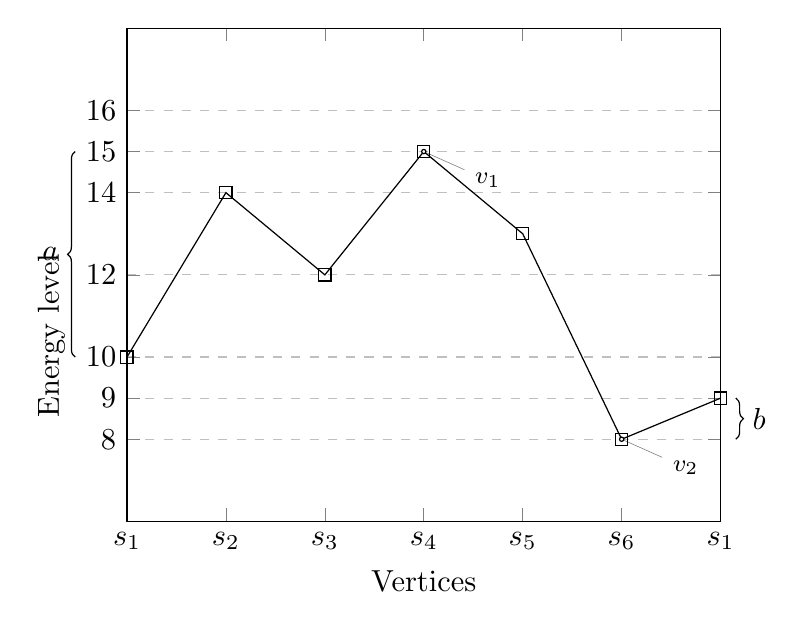
\begin{tikzpicture}[scale=1.1]
\begin{axis}[
    title={},
    xlabel={Vertices},
    ylabel style= {xshift=-20pt},
    ylabel={Energy level},
    clip=false,
    xmin=1, xmax=7,
    ymin=6, ymax=18,
    xtick={1,2,3,4,5,6,7},
    ytick={8,9,10,12,14,15,16},
    xticklabels={$s_1$,$s_2$,$s_3$,$s_4$,$s_5$,$s_6$,$s_1$},
     legend pos=north east,
    ymajorgrids=true,
    grid style=dashed,
]

\addplot[
    color=black,
    mark=square,
    ]
    coordinates {
    (1,10)(2,14)(3,12)(4,15)(5,13)(6,8)(7,9)
    }; 

\node[inner sep=0.5pt,circle,draw,fill=white,pin=-15:\footnotesize $v_1$] 
	  at (axis cs:4,15) {};
	  \node[inner sep=0.5pt,circle,draw,fill=white,pin=-15:\footnotesize $v_2$] 
	  at (axis cs:6,8) {};


\draw[decorate,decoration={brace}]
  ([xshift=-17pt]axis cs:1,10) --
    node[left=2pt] {$a$} 
  ([xshift=-17pt]axis cs:1,15);

\draw[decorate,decoration={brace,mirror}]
  ([xshift=5pt]axis cs:7,8) --
    node[right=2pt] {$b$} 
  ([xshift=5pt]axis cs:7,9);
\end{axis}
\end{tikzpicture}
\caption{Energy level of a negative cycle}

  \end{figure}
  \vskip 0.1cm
  In the example, $U=15$. Hence, $a=5$ and $b=1$, i.e. if player $1$ can reach $s1$ with at most 10 energy level, he can rotate the cycle as much as he wants, and can get the energy level down to energy 1.\\
  Consider a winning path $\rho$ in $G$. Suppose a negative cycle $C$ exists in that path. That means, the path visits the vertex $v_1$, the point with the highest energy level in $C$ at least once. As, the path is winning, it visits $v_1$ with energy level $\leq U$. Hence, if we can compute $(U,b)$ for that vertex $v_1$, we can say that, after visiting the cycle $C$, $P_1$ can rotate around the cycle and get the energy level down to $b$ at $v_1$. Using the idea, we can do the following:\\
  \begin{itemize}
  \item For every vertex $v$, we will check, if it is the highest point of any negative cycle i.e. will check if pair $(U,b)$ exists for some $b \in \mathbb{N} \cup \{0\}$. If yes, then we will calculate the optimal $b$.
  \item We will fill the table $H_{vertex \times steps}$ such that, $H(v,i)=$ The minimum energy level we can have at $v$ after at least $i$ - steps starting from $q_0$. 
  \end{itemize}
  \vskip 0.1cm
  Notice that, if $(U,b)$ pair exists for a vertex $v$, there must exist a negative edge out of it. From the above observation about the energy levels of a negative cycle, it is easy to see that, if $(U,b)$ exists for $v$, from $v$, along the negative cycle, there will be a vertex $u$, where the energy level will be minimum, say $x$. Similarly, there must be a positive weight edge out of $t$. Then, starting from $t$, there will be a path back to $v$. Hence, for every vertex $v$, which has at least one negative edge out of it, we will start with energy level $U$, and for every other vertex $t$ with at least one positive weight edge out of it, we will try to find, if there exists a path of at most length $|V|$, such that it reaches $t$ maintaining the strict upper and the weak lower bound, with energy level $x$, and along the path the energy level never goes below $x$. If we can find such vertex $t$, with energy level $x$, similarly we will try to find, starting from $t$ with $x$ energy, do we have a path of length at most $|V|$ back to $v$, maintaining all the bounds and also such that $x$ is the minimum energy level along the path. Let, we reach $v$ with energy $y$. Then, $b=y-x$. If, we find several such $b$, we will take the minimum one as the optimal. Both the path-checking can be done by simple DFS maintaining the energy level with the vertices. We stop at each path in the DFS when the bound is violated or the length of the path becomes $|V|$. We can also, maintain a counter to remember the minimum energy level seen along the path. Hence, we can compute $(U,b)$ pair for vertices, if exists, in polynomial time.\\
  \vskip 0.1cm
  Once, we have computed the $(U,b)$ pairs for vertices, we can add the following special edges in the graph:\\
  If $(U,b)$ exists for $v$, we add a special loop $v \xrightarrow{\text{:=b}} v$ in the game graph. The idea is, if player $1$ can reach $v$ with at most $U$ energy, he can take some negative cycle in the original graph and get the energy level to $b$ after sufficient many steps. In this new graph, player $1$ can take this special loop and in one step he can lower the energy level of $v$, down to $b$ at one step. Clearly, player $1$ can win in the original graph iff he can win in this new graph with the special transitions.\\
  Now, in this special graph, we will calculate the table $H_{vertex \times steps}$. For any vertex $v$, let \\$e_i=min\{H(u,i-1) + w(u,v) | (u,v)\in E\  \&\  H(u,i-1) \leq U\}$. Then,
   $$
   H(v,i)=
   \begin{cases}
    min(e_i,b), \hskip 0.5cm &\text{if $v \xrightarrow{\text{:=b}} v$ exists and
    $H(v,i-1) \leq U$}\\ 
   e_i, \hskip 1cm &\text{otherwise}
 \end{cases}
 $$
 Now, if for some $i$, $H(T,i)\leq U$, player $1$ wins, otherwise, he loses.\\
 \vskip 0.1cm
 Consider a winning path $\rho$ for player $1$. We have already argued that, there is no positive cycle in this path. Now, the claim is, every special loop can appear at most once in $\rho$. This can be easily seen as the following:\\
 Let, same special transition appears twice in the winning path $\rho$ at $i^{th}$ and $j^{th}$ positions.\\
 \begin{figure}[htb]
 \hskip 2cm
  \begin {tikzpicture}[-latex ,auto ,node distance =1 cm,
 state/.style ={ circle ,top color =white , bottom color = processblue!20 ,
 draw,processblue , text=blue , minimum width =1 cm}]

 \node[state] (A) [] {$q_0$};
 \node[state,label=above:{$i$}] (B) [right= 4cm of A] {$v$};
 \node (01) [right =1cm of B] {$$};
 \node[state,label=above:{$j$}] (C) [right=2.5cmof B] {$v$};
 \node (02) [right =1cm of C] {$$};
 \node[state] (D) [right=4cmof C] {$T$};

 \path (A) edge [dashed] node[above =0.15 cm] {$$} (B);
 \path (B) edge [] node[above =0.15 cm] {$:=b$} (01);
 \path (C) edge [] node[above =0.15 cm] {$:=b$} (02);
 \path (01) edge [dashed] node[above =0.15 cm] {$$} (C);
 \path (02) edge [dashed] node[above =0.15 cm] {$$} (D);
 \end{tikzpicture}
 
 \end{figure}
 \vskip 0.1cm
 Then, the configuration of the path $\rho$ in both the positions are same. Hence, player $1$ can just forget the middle part between the positions, and continue similarly from the $i^{th}$ position, as progressed from the $j^{th}$ position. As, the original path is winning, the new truncated path will also be winning for player $1$.\\
 Now, to prove the correctness of the algorithm proposed earlier, it is enough to prove the following lemma:\\
 \vskip 0.1cm
 \begin{lemma}
 \label{poly-lemma}
  If there exists a winning path for player $1$ in $G$, there exists a winning path of length at most $|Q|^2$ for player $1$.
  \end{lemma}
  \vskip 0.1cm
  \textit{Proof of Lemma \ref{poly-lemma}} Let the optimal shortest winning path for player $1$ has length $>|V|^2$. By pigeon hole principle, $\exists u \in Q$, which appears in the path $|Q|+1$ times. Therefore the path has admitted at least $|Q|+1$ cycles through $u$. As, there can not be any positive cycle in the optimal winning path, all of them are negative cycles. For every negative cycles, the will admit a special transition of the form $v \xrightarrow{\text{:=b}} v$ as shown earlier. Hence, there exists at least $|Q|+1$ special transitions in the path. But the number of unique special transitions are bounded by $|Q|$ and we know, each special transition can appear at most once in the optimal path. Then the contradiction arises\\
 \vskip 0.3cm
  From Lemma \ref{poly-lemma}, it is evident that, calculating $H_{vertex \times steps}$ up to at most $|Q|^2$ many steps are enough.\\
  This completes the proof for our theorem.
 \end{proof}
 \vskip 0.1cm
 Now, we will move to the case for the two player version.
 
 
\section{Two Player QR Games with Weak Dual Bounds}

Now, $Q_2 \not = \phi$ anymore. We will first prove the following lemma about the memory requirements for both the players in the game.\\
\begin{lemma}
\label{mem-lemma}
For two player QR games with weak dual bounds, exponential memory may be necessary for player $1$. For player $2$, memoryless strategies are sufficient.
\end{lemma}
\begin{proof}
As reachability is one of the objective, trivially finite memories are sufficient for both the players. Now, we will show, a class of game graphs, where exponential memory may be necessary for player $1$.\\
\begin{figure}[htb]
\hskip 6cm
\label{expmem-p1}
\begin {tikzpicture}[-latex ,auto ,node distance =1 cm,
state/.style ={ circle, draw, minimum width =1 cm, jaune}]

\node[state] (A) [] {$q_0$};
\node[state] (B) [right=of A] {$v$};
\node[state] (C) [right=of B] {$T$};

\path (A) edge [] node[above =0.15 cm] {$0$} (B);
\path (B) edge [loop above] node[above =0.15 cm] {$+1$} (B);
\path (B) edge [] node[above =0.15 cm] {$-W$} (C);
\end{tikzpicture}
\caption{Exponential memory is necessary for player $1$ }


\end{figure}

In the game graph of Figure \ref{expmem-p1}, all the vertices are player $1$  vertices and $U$ is the strict upper bound. It is easy to see, player $1$ needs at least $U$- memory to win this game. Considering binary encoding. the value of $U$ is exponential in the size of the input.\\
Now, we will prove that, memoryless strategies are enough for player $2$. Let's fix a winning strategy $lambda$ for player $2$  WLOG, every player $2$ vertices have two outgoing ages. Fix one player $2$ vertex, say $q_2$. Let the weight of the two outgoing edges from $q_2$ are $e_l$ and $e_r$ to $q_l$ and $q_r$ respectively. Now, if any path reaches $q_l$ with at most $w_l$ energy, player $1$ can win from $q_l$ and similarly if any path reaches $q_r$ with at most $w_r$ energy, player $1$ can win from $q_r$. Clearly, if any path reaches $q_2$ with at most $min(w_l-e_l, w_r-e_r)= w^{\prime}$,say, energy, no matter what player $2$ chooses from $q_2$, player $1$ wins. As, $\lambda$ is winning for player $2$, no outcome of $\lambda$ reaches $q_2$ with $\leq w^{\prime}$ energy. W.L.O.G., let $w^{\prime}= w_l -e_l$. It is easy to see that, we can construct a memoryless strategy $\lambda^{\prime}$ for player $2$, such that $\lambda^{\prime}(q_2)=q_l$. Hence, memoryless strategy is enough for player $2$.
\end{proof}
 
\chapter{Apna Game}
In the previous chapters, we have explored all kind of weighted games, where the weight functions were bounded. In this chapter, we will explore a new kind of a game. Here also, we have strong bounds on weights, but player $1$ can violate one of the bounds, w.l.o.g, say the upper bound. The number of vertices, he traverses along his path with weights higher than the upper bound are called \textbf{violations}. In this game, we have a bound on the number of violations. We call this bounded violations reachability game as \textit{Apna Game}. We formally define it in the following section.\\

\section{Description of the Game}
Consider a game graph $G=\langle Q_1, Q_2, E, w, q_0, T \rangle$, a lower bound $l$, an upper bound $U$ and a 

\chapter{Conclusion}
In this thesis, we have considered several variants of energy games. The first variant defines games with upper and lower bound constraints, combined with reachability or infinite runs objectives. 
The second variant proposed defines games with a strong lower bound and a relaxed upper bound that can be weak or temporarily exceeded, combined with reachability or infinite run objectives, and constraints on violations of upper bound. 
\vskip 0.3cm
In the one player case, complexities ranges from PTIME to PSPACE-Complete. and in the two-player case from NP $\cap$ coNP to EXPTIME-Complete. 
In general, the complexity is the same for a reachability and for an infinite run objective. Interestingly, for \LWenergy games, the complexity of the single player case is PTIME, but reachability objectives require exponential memory (in the size of the weak upper bound) while strategies are memoryless for infinite run objectives.
\vskip 0.3cm
Table~\ref{table-results} summarizes known
results, and the results obtained in this paper (where \LVenergyall
gathers all three energy constraints with violations). We furthermore show that the minimization problem for \LVenergyall (reachability) games require algorithms that run in PSPACE in the one-player case, and in EXPTIME in the two-players case.


\begin{table}[ht]
  \centering
  \def\arraystretch{2}
  \def\comp{c.}
  \scalebox{0.7}{
  \begin{tabular}{|c||c|c||c|c|}
    \hline
    &\multicolumn{2}{c|}{Reachability}&\multicolumn{2}{c|}{Infinite runs}\\
    \hline
    & 1 player & 2 players & 1 player & 2 players
    \\\hline\hline
    \Lenergy & PTIME~(thm.~\ref{thm_reachability_games})&NP$\cap$ coNP~(thm.~\ref{thm_reachability_games}) 
    & PTIME~\cite{BouyerFLMS08} & in NP $\cap$ coNP~\cite{BouyerFLMS08}\\\hline
    %LUEnergy Games
    \LUenergy&PSPACE-\comp~(thm.~\ref{pspace-complete})& EXPTIME-\comp ~(thm.~\ref{exp-complete})
    & PSPACE-\comp~\cite{BouyerFLMS08} &EXPTIME-\comp~\cite{BouyerFLMS08}\\\hline
    %
    \LWenergy&PTIME~(thm.~\ref{one-player-weak-thm})&coNP~(thm.~\ref{two-player-weak-thm}) 
    &PTIME~\cite{BouyerFLMS08} &NP $\cap$ coNP~\cite{BouyerFLMS08}\\\hline
    %
    APNA$^{*}$-games &PSPACE-\comp~(thm.~\ref{thm_apna_LUHV_2P}) &EXPTIME-\comp~(thm.~\ref{thm_apna_LUHV_2P})&PSPACE-\comp~(thm.~\ref{thm_apna_LUHV_2P}) &EXPTIME-\comp~(thm.~\ref{thm_apna_LUHV_2P}) \\\hline
    
    
    Bound existence&PSPACE-\comp~(thm.~\ref{thm_Apnar_exists_min_exptimec})&EXPTIME-\comp~(thm.~\ref{thm_Apnar_exists_min_exptimec}) &PSPACE-\comp~(thm.~\ref{thm_Apnar_exists_min_exptimec})&EXPTIME-\comp~(thm.~\ref{thm_Apnar_exists_min_exptimec}) \\\hline
  \end{tabular}
  }
  \caption{Summary of the results}
  \label{table-results}
\end{table}
\vskip 1cm
A possible extension of this work is to consider energy games with mean payoff function and discounted total payoff for the energy level and for the violation constraints, and the associated minimization and existence problems. 




\bibliographystyle{alpha}
\bibliography{Thesis}

\appendix
\chapter{Appendix Title}
\section{Proofs of Section~\ref{sec-weak}}

\noindent{\bf Lemma \ref{lemma-higherrun}: }
  Let $\pi$ be a finite path in a one-player arena~$G$.
  If $(q,u) \xrightarrow{\pi}_{LW} (q',u')$,
  then for any~$v\geq u$,
  $(q,v) \xrightarrow{\pi}_{LW} (q',v')$ for some~$v'\geq u'$.

\begin{proof}
Write $\pi=(e_i)_{0\leq i<n}$, with $e_i=(q_i,p_i,q'_i)$ for each~$i$.
The sequence defined as
\begin{xalignat*}2
  u_0&= u & u_{i+1} &= \min{W,u_i+p_i}
\end{xalignat*}
is the sequence of energy levels along the run $(q,u) \xrightarrow{\pi}_{LW}
(q',u')$.  For~$v\geq u$, letting
\begin{xalignat*}2
  v_0&= v & v_{i+1} &= \min{W,v_i+p_i},
\end{xalignat*}
we~easily prove by induction that for all~$i$, $u_i\leq v_i\leq W$,
which entails that $(q,v) \xrightarrow{\pi}_{LW} (q',v')$ with $v'=v_n\geq
u_n=u'$.
\end{proof}


\noindent{\bf Proof of Lemma~\ref{lemma-hitW}}
  Let $\pi$ be a finite path in a one-player arena~$G$, and consider two LW-runs 
  $(q,u)\xrightarrow{\pi}_{LW} (q',u')$ and $(q,v)\xrightarrow{\pi}_{LW}(q',v')$ with $u\leq
  v$. Then $u'-u\geq v'-v$, and if the inequality is strict, then
  the energy level along the run $(q,v)\xrightarrow{\pi}_{LW}(q',v')$ must have hit~$W$.


\begin{proof}
  The first statement is proven by induction: we~again write
  $\pi=(e_i)_{0\leq i<n}$, with $e_i=(q_i,p_i,q'_i)$ for each~$i$, and
  \begin{xalignat*}2
    u_0&= u & u_{i+1} &= \min(W,u_i+p_i)\\
    v_0&= v & v_{i+1} &= \min(W,v_i+p_i).
  \end{xalignat*}
  Then $u_{i+1}-u_i=\min(W-u_i,p_i)$ and
  $v_{i+1}-v_i=\min(W-v_i,p_i)$.  Since $u_i\leq v_i$ for all~$i$,
  we~also have $W-u_i\geq W-v_i$, and $u_{i+1}-u_i \geq
  v_{i+1}-v_i$. By~summing up these inequalities, we~get $u_{i+1}-u_0
  \geq v_{i+1}-v_0$. Now, as long as $W-v_i\geq p_i$ (then also
  $W-u_i\geq p_i$), the inequalities above are equalities. It~follows
  that if the inequality is strict, then the run
  $(q,v)\xrightarrow{\pi}_{LW}(q',v')$ must have hit~$W$.
\end{proof}


\noindent{\bf Proof of Lemma~\ref{lemma-W}}
Let $\pi$ be a finite path in a one-player arena~$G$, for which there
  is an LW-runs $(q,u)\xrightarrow{\pi}_{LW} (q',u')$. 
  %with $u\leq u'$. (suppressed this info otherwise the second statement makes no sense) 
  If $u'$ is the maximal energy level along that run, then
  $(q,W)\xrightarrow{\pi}_{LW} (q',W)$;
  if $u$ is the maximal energy level along the run above, then
  $(q,W)\xrightarrow{\pi}_{LW} (q',W+u'-u)$.


\begin{proof}
  Write $\pi=(e_i)_{0\leq i<n}$, with $e_i=(q_i,p_i,q'_i)$ for
  each~$i$. If~$u'$ is the maximal energy level, then for all~$i$,
  we~have $\sum_{j=i}^{n-1} p_j\geq 0$.  Now, define
  \begin{xalignat*}2
    v_0&= W & v_{i+1} &= \min(W,v_i+p_i).
  \end{xalignat*}
  If~$v_n<W$, then by induction we also have $v_i<W$ for all~$i$,
  contradicting the fact that~$v_0=W$. This proves our first result.

  Similarly, if~$u$ is the maximal energy level, then for all~$i$,
  we~have $\sum_{j=0}^{i} p_j\leq 0$. Then for all~$i$,
  $v_{i+1}=v_i+p_i\leq W$, so that $v_{n}-v_0=u'-u$. Our second result
  follows.
\end{proof}


\noindent{\bf Proof of Lemma~\ref{lemma-iteratepos}}
Let $\pi$ be a finite path in a one-player arena~$G$.
  If
  $(q,u)\xrightarrow{\pi}_{LW} (q',u')$ with $u'> u$
  and 
  $(q,w)\xrightarrow{\pi}_{LW} (q',w')$ with $w'> w$,
  then
  for any $u\leq v\leq w$, it~holds
  $(q,v)\xrightarrow{\pi}_{LW} (q',v')$ with $v'> v$.

\begin{proof}  
Using Lemma~\ref{lemma-higherrun}, we~immediately have
$(q,v)\xrightarrow{\pi}_{LW} (q',v')$. As~in the previous proof, we~define
sequences
\begin{xalignat*}2
  u_0&= u & u_{i+1} &= \min(W,u_i+p_i)\\
  v_0&= v & v_{i+1} &= \min(W,v_i+p_i)\\
  w_0&= w & w_{i+1} &= \min(W,w_i+p_i).
\end{xalignat*}
We~still have $u_i\leq v_i\leq w_i$ for all~$i$. Moreover, 
%if $v_j<M$
if $v_j<\wub$
for all~$j\leq i$, then $v_i-u_i=v-u$. As~a consequence, if $v'\leq
v$, then it must be the case that 
%$v_j=M$ 
$v_j=\wub$ 
for some~$j$; but then $w_j=v_j$, 
%since $v_j\leq w_j\leq M$. 
since $v_j\leq w_j\leq \wub$. 
It~follows that $w_k=v_k$ for
all~$k\geq j$, so at the end of $\pi$ we have $w'=v'$. Assuming $v'\leq v$ raises a contradiction since we have $v'=w'>w\geq v$.
%This is a contradiction, since we assumed $v'\leq v$ and have $w'>w$ by hypothesis. 
Hence $v'>v$.
\end{proof}

\noindent{\bf Proof of Lemma~\ref{lemma-removeneg}}
Let $\pi$ be a finite path in a one-player arena~$G$.
  If $(q,u) \xrightarrow{\pi}_{LW} (q',u')$ and $\pi$ can be decomposed as
  $\pi_1\cdot\pi_2\cdot \pi_3$ in such a way that
  $(q,u) \xrightarrow{\pi_1}_{LW}
%  (s,v)\LWarrow{\pi_2}(s',v') \LWarrow{\pi_3}(q',u')$ with $v'\leq
  (s,v)\xrightarrow{\pi_2}_{LW}(s,v') \xrightarrow{\pi_3}_{LW}(q',u')$ with $v'\leq
  v$, then $(q,u)\xrightarrow{\pi_1\cdot\pi_3}_{LW} (q',u'')$ with $u''\geq
  u'$.

\begin{proof}
%Since $(s',v') \LWarrow{\pi_3}(q',u')$ and $v'\leq v$, by
Since $(s,v') \xrightarrow{\pi_3}_{LW}(q',u')$ and $v'\leq v$, by
Lemma~\ref{lemma-higherrun} 
%we also have $(s',v)
we also have $(s,v)
\xrightarrow{\pi_3}_{LW}(q',u'')$ for some~$u''\geq u'$. The~result follows.
\end{proof}


\noindent{\bf Proof of Lemma~\ref{lemma-iteratecycles}}
Let $\pi$ be a cycle on~$q$ such that $(q,u) \xrightarrow{\pi}_{LW} (q,v)$
  for some $u\leq v$. Then $(q,u) \xrightarrow{\pi^{W-L}}_{LW} (q,v')$ for
  some~$v'$, and $(q,v')\xrightarrow{\pi}_{LW} (q,v')$.


\begin{proof}
  The case where $u=v$ is trivial. We~assume $u<v$.  Applying
  Lemma~\ref{lemma-higherrun} inductively, we get that the cycle can
  be iterated arbitrarily many times; this~also proves that the
  sequence of energy levels reached at the end of each iteration is
  non-decreasing.

  Now, assume that $(q,v')\xrightarrow{\pi}_{LW} (q,v'')$ for
  some~$v''\not=v'$.  Then $v''>v'$. Lemma~\ref{lemma-iteratepos} then
  entails that the sequence of energy levels reached at the end of
  each iteration is increasing. Since the loop has been iterated $W-L$
  times, the~energy level in~$v''$ would exceed~$W$, which is
  impossible. This proves our result.
\end{proof}


\noindent{\bf Proof of Lemma~\ref{lemma-DAGlabel}}
  Let~$[q,d]$ be a state of the DAG, and $M$ and~$m$ be two integers
  such that $0\leq m\leq M$.  Upon termination of this algorithm, 
  state~$[q,d]$ of the DAG is labelled with~$(M,m)$ if, and only if,
  there is an LW-run of length~$d$ from~$(q_0,L)$ to~$(q,M-m)$ along
  which the energy level always remains in the interval~$[L,M]$.

\begin{proof}
  The proof is by induction on~$d$. The result is trivial for~$d=0$.
  Now, assume it holds for some depth~$d-1$, and pick a
  state~$[q,d]$. For the first direction, if~$[q,d]$ is labelled
  with~$(M,m)$, then this label was added using some
  transition~$([q',d-1],w,[q,d])$ and some label~$(M',m')$
  of~$[q',d-1]$. By~induction, there is an LW-run~$\rho$ of
  length~$d-1$ from~$(q_0,L)$ to~$(q',M'-m')$ in~$G$ along which the
  energy level remains in the interval~$[L,M']$. We~consider two cases,
  corresponding to the two ways of updating the pair of values:
  \begin{itemize}
  \item if $w>m'$, then we~have $M=min(\wub,M'-m'+w)$ and $m=0$. %$M=\max(W,M'-m'+w)$ and $m=0$. 
  Now, the transition $([q',d-1],w,[q,d])$ in the DAG originates from a
    transition~$(q',w,q)$ in~$G$; taking this transition after~$\rho$
    provides us with the run of length~$d$ from~$(q_0,L)$ to~$(q,M-m)$
    along which the energy level remains in~$[L,M]$, as required;
  \item if $m'+L-M'\leq w\leq m'$, then $M=M'$ and $m=m'-w$. Again,
    taking transition~$(q',w,q)$ after~$\rho$ provides us with the
    LW-run we are looking for.
  \end{itemize}

  Conversely, if there is an LW-run~$\rho$ of length~$d$
  from~$(q_0,L)$ to~$(q,M-m)$ along which the energy level always
  remains in the interval~$[L,M]$, then we~write $\rho=\rho'\cdot
  ((q',l'),w,(q,M-m))$, distinguishing its last transition. By~induction, $[q',d-1]$ must have been labelled with a pair~$(M',m')$ such that $l'=M'-m'$ and the energy level
  along $\rho'$ remained within $[L,M']$. Now, from the existence of a transition $((q',l'),w,(q,M-m))$, we~know that there is a
  transition~$([q',d-1],w,[q,d])$ in the~DAG, which will generate the required label of~$[q,d]$.
\end{proof}

\noindent{\bf Proof of Lemma~\ref{lemma-univcycle}}
  Let~$[q_0,d]$ be a state of the DAG, with~$d>0$. Let $m$ be a
  non-negative integer such that $L<W-m$.  Upon termination of this algorithm, state~$[q_0,d]$ is labelled with~$(M,m)$ such that $M-m>L$ if, and only if, there is a universal  positive cycle~$\phi$ on~$q_0$ of length~$d$ such that $(q_0,L) \xrightarrow{\phi^{W-L}}_{LW} (q_0,W-m)$.

\begin{proof}
First assume that~$[q_0,d]$ is labelled with~$(M,m)$ for some~$M$ such
that $M-m>L$. From Lemma~\ref{lemma-DAGlabel}, there is a cycle~$\phi$
on~$q_0$ of length~$d$ generating a run $(q_0,L)\xrightarrow{\phi}_{LW}(q_0,M-m)$
along which the energy level is within~$[L,M]$.  Then~$M-m\geq L$, so
that Lemma~\ref{lemma-iteratecycles} applies: we~then get $(q_0,L)
\xrightarrow{\phi^{W-L}}_{LW} (q_0,E)$ with $(q_0,E)\xrightarrow{\phi}_{LW}(q_0,E)$.
Write $(p_i)_{0\leq i<|\phi|}$ for the sequence of weights along~$\phi$.
Also write $\rho$ for the run $(q_0,L)\xrightarrow{\phi}_{LW}(q_0,M-m)$, and
$\sigma$ for the run $(q_0,E)\xrightarrow{\phi}_{LW}(q_0,E)$.

%Assume $L=M-m$: iterating~$\phi$ would not modify the energy level
%reached at the end of those cycles, so that we would have
%$L=W-m$. Since this is not the case, it~must be 
As $L<M-m$, then by Lemma~\ref{lemma-hitW}, it~must be the case that energy level~$W$ is
reached along~$\sigma$.  Write~$i_0$ and $j_0$ for the first and last
positions along~$\rho$ for which the energy level along~$\rho$ is~$M$.
That is, the subpath from index $0$ to index $i_0$ has growing energy level, and the subpath from $j_0$ to $|\rho|$ has a decreasing energy level. 
Assume $\tilde\sigma_{i_0}\not=W$: by~Lemma~\ref{lemma-higherrun},
we~must have $M=\tilde\rho_{i_0}\leq \tilde\sigma_{i_0}<W$.  Then for
all~$k\geq i_0$, $\sum_{l=i_0}^k p_l\leq 0$, and $\sum_{l=i_0}^{j_0}
p_l= 0$. Since $\tilde\sigma_{i_0}<W$, then also $\tilde\sigma_{k}<W$
for all~$k\geq i_0$. According to Lemma~\ref{lemma-hitW}, energy level $\wub$ is reached in $\sigma$, so 
%HERE 
there exists some~$k_0<i_0$ such that $\tilde\sigma_{k_0}=W$;
%$\tilde\rho_{k_0}<M$, 
However, as $i_0$ is the index of the first maximal value in $\rho$, we have $\tilde\rho_{k_0}<M$, and the energy level increases in run $\rho$ between $k_0$ and $i_0$. So according to Lemma~\ref{lemma-W}, we should have $\tilde\sigma_{i_0}<W$, which raises a contradiction.
Hence we proved $\tilde\sigma_{i_0}=W$; applying
the second result of Lemma~\ref{lemma-W}, we~get $E=W-m$.

\medskip
Conversely, if there is a universal positive cycle~$\phi$ satisfying the
conditions of the lemma, let $F$ be such that $(q_0,L)\xrightarrow{\phi}_{LW}
(q_0,F)$, and~$M$ be the the maximal energy level encountered along
the run $(q_0,L)\xrightarrow{\phi}_{LW} (q_0,F)$. By
Lemma~\ref{lemma-DAGlabel}, state~$[q_0,d]$ is labelled with~$(M,m')$
for some~$m'\geq 0$ such that $F=M-m'$.
By~Lemma~\ref{lemma-iteratecycles}, we~must have $(q_0,L)
\xrightarrow{\phi^{W-L}}_{LW} (q_0,W-m')$.
%, so that $m'=m$.
\end{proof}


\noindent{\bf Proof of Lemma~\ref{lemma-order-cycle}}
Consider two paths~$\pi$ and~$\pi'$ such that
$first(\pi)=first(\pi')$ and $last(\pi)=last(\pi')$, and with
respective values~$(M,m)$ and~$(M',m')$ such that $(M,m)\preceq (M',m')$.
If~$\pi$ is a prefix of a universal cycle~$\phi$, then $\pi'$~is a
prefix of a universal cycle~$\phi'$ with $\phi'\triangleright\phi$.

\begin{proof}
  Let $q=first(\pi)$ and $q'=last(\pi)$.  We~write~$\psi$ for the
  path such that $\phi=\pi\cdot\psi$; $\psi$~is a path from~$q'$
  to~$q$. Then $(q,L)\xrightarrow{\pi}_{LW} (q'',M-m)
  \xrightarrow{\psi}_{LW}(q',F)$. Also, $(q,L)\xrightarrow{\pi}_{LW} (q'',M'-m')$.  Since
  $M-m\leq M'-m'$, we have $(q'',M'-m')\xrightarrow{\psi}_{LW}(q',F')$. We~can
  thus let $\phi'=\pi'\cdot\psi$: by~Lemma~\ref{lemma-univcycle},
  the~final energy level reached after iterating~$\phi'$ is higher
  than the energy level reached after iterating~$\phi$, since $m'\leq
  m$. Hence $\phi'\triangleright\phi$.
\end{proof}



\noindent{\bf Proof of Lemma~\ref{lemma-DAG-construction-poly}}
%If in our algorithm we only store maximal labels (for~$\preceq$), then
%the algorithm runs in polynomial time.
If the DAG construction algorithm only stores maximal labels (for~$\preceq$), then
it runs in polynomial time.

\begin{proof}
We prove that, when attaching to each node $[q,d]$ of the DAG only the maximal labels (w.r.t $\preceq$) reached for a path of length $d$ ending in state $q$, the number of
values for the first component of the different labels that appear at
depth~$d>0$ in the DAG is at most $d\cdot |Q|$. Since it only
stores optimal labels, our algorithm will never associate to a state $[q,d]$
two labels having the same value on their first component. So, any
state at depth~$d$ will have at most $d\cdot |Q|$ labels.

So we prove, by induction on~$d$, that the number of different values
for the first component among the labels appearing at depth~$d>0$ is
at most~$d\cdot|Q|$. 
%
This is true for~$d=1$ since the initial state~$(q,0)$ only
contains~$(M=0,m=0)$, and each transition with nonnegative weight~$w$
will create one new label~$(w,0)$ (transitions with negative weight
are not prefixes of universal cycles). Now, since all those labels
%have the same value on their second component,
have value 0 as second component, each state $[q,1]$ in the DAG will be attached at most one label. Hence, the total number of labels (and the total number of different values for their first
component) is at most~$|Q|$ at depth 1 in the DAG.

Now, assume that the labels appearing 
%at depth~$q$ 
at depth $d>1$ are all drawn from a set of labels~$L=\{M_i,m_i) \mid 1\leq i\leq n\}$ in which the
number of different values of~$M_i$ is at most $d\cdot|Q|$.
Consider a state~$[q',d]$, labelled with $\{(M_i,m_i) \mid 1\leq i\leq
n_{q',d}\}$ (even if it means reindexing the labels). Pick~a
transition from~$[q',d]$ to~$[q'',d+1]$, with weight~$w$. For each
pair~$(M_i,m_i)$ associated with $[q,d]$, it~creates a new label in~$(q'',d+1)$; this label
is
\begin{itemize}
\item either $(M_i-m_i+w,0)$ if~$m_i<w$;
\item or $(M_i,m_i+w)$ if $m_i=M_i\leq w\leq m_i$.
\end{itemize}
Now, for a state~$(q'',d+1)$, the~set of labels created by all
incoming transitions can be grouped as follows:
\begin{itemize}
\item labels having~zero as their second component; among those, our
  algorithm only stores the one with maximal first component, as $(M_i,0) \preceq (M_j,0)$ as soon as $M_i\leq M_j$;
\item for each $M_i$ appearing at depth~$d$, labels having~$M_i$ as
  their first component; again, we only keep the one with minimal
  second component, as $(M,m_i) \preceq (M,m_j)$ when $m_j \leq m_i$.
\end{itemize}
In~the end, for this state~$[q'',d+1]$, we keep at most one label for
each distinct value among the first components $M_i$ of labels appearing at depth~$d$, and possibly one extra
label with second value~$0$. In~other terms, at depth $d+1$ the values that appear as first component of labels are 
obtained from values at depth~$d$, plus possibly one per state; Hence, at depth $d+1$, there exists at most $(d+1)\cdot|Q|$ labels, which completes the proof of the induction step.\qed
\end{proof}



\noindent{\bf Proof of Lemma~\ref{lemma-higherstrat}}
  Let $G$ be a two-player arena, equiped with an \LWenergy-reachability
  objective. Let~$q$ be a state of~$G$, and~$u\leq u'$ in $[L;W]$. If
  \Pl1 wins the game from~$(q,u)$, then she also wins from~$(q,u')$.

\begin{proof}
Let~$\sigma$ be a winning strategy for \Pl1 from~$(q,u)$. If she plays
the same strategy from~$(q,u')$, then for any strategy of~\Pl2, the
resulting outcome from~$(q,u')$ follows the same transitions as the
outcome of the same strategies from~$u$, with higher energy
level. Since~$\sigma$ is winning from~$(q,u)$, it~is also winning
from~$(q,u')$.
\end{proof}

\end{document}
